%!TEX root=paper.tex

\newpage
\section{The System}

For the long term, we envision an open educational ecosystem in which different creators can integrate their applications by interacting with a core API that provides the basic contextual translations, user knowledge estimation, and recommendations for words to be studied and texts to be read \cite{Lungu16}. 

However, in order to bootstrap, experiment with, and show the potential of such an ecosystem, we present here our basic implementation of each of the components. In particular we describe our own implementation of: 

\begin{description}

  \item [Text Recommender] -- which consists of a feed subscription mechanism, an article browser that presents the results of crawling the selected feeds that the user is interested in

  \item [Text Reader] -- which is a web-based interactive text reader which provides seamless in place translations
  
  \item [Vocabulary Trainer] -- which consists of an exercise platform which generates exercises based on a reader's past reading experience

\end{description}

The components that we present here are implemented using HTML5 and Javascript technologies for the front end and Python and Flask for the backend. For the frontend, we have experienced in the past with writing native applications, however, the interaction with the native elements was too clumsy. Moreover, maintaining multiple systems for multiple platforms is too expensive for an academic environment. The decision turned out to be practical since the users of our system come from multiple platforms.


\subsection{The Text Recommender}
\ml{make sure that this flows well for the reader while also keeping it short}
The reading recommender is simple at the moment. It consists of a Feed Subscription and an Article Browser.

\subsubsection{Feed Subscription}
When the user indicates that they would like to subscribe to a new source, as explained above, the subscription dialog is displayed. Zeeguu categorizes feeds by their language, and thus we allow users to select any language available and retrieve a list of that language's sources. Languages are represented by flags, as their compact and iconic representation should be universally understood.

\begin{figure}[h!]
\centering
  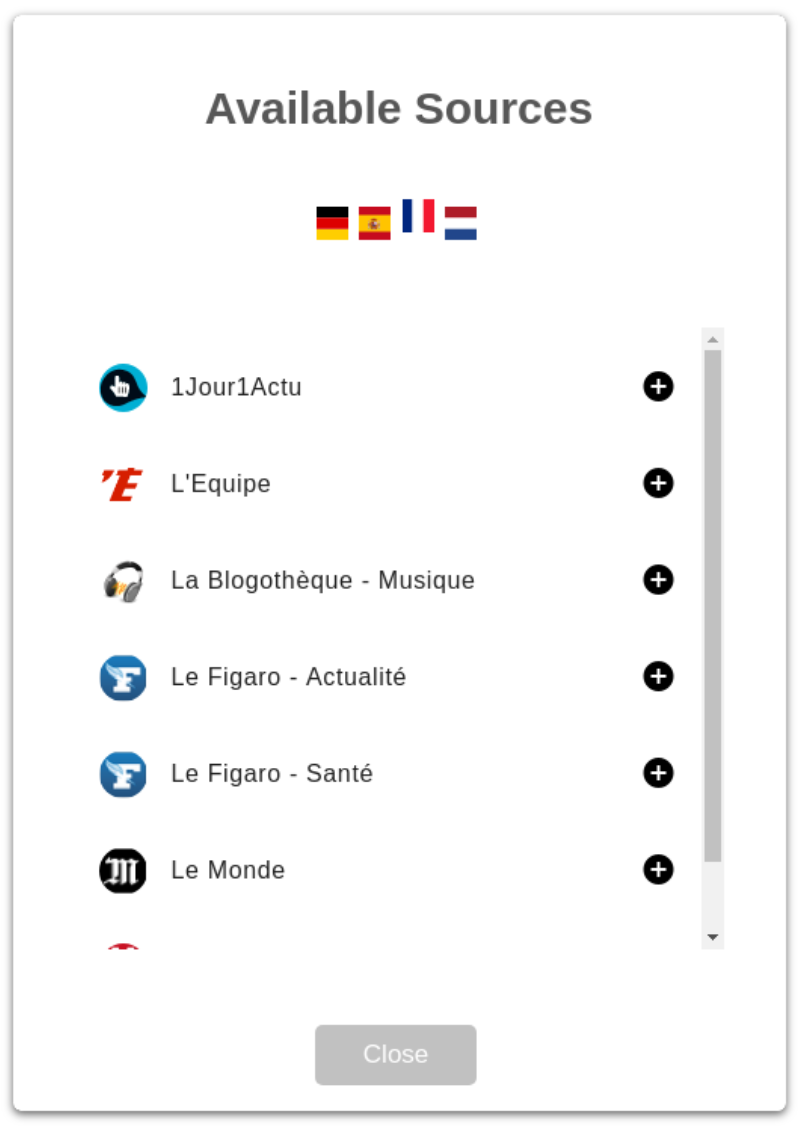
\includegraphics[width=0.4\columnwidth]{figures/available_sources}
  \caption{Different users subscribe to different sources}~\label{fig:registrations}
\end{figure}


\subsubsection{Article Browser}

Article listing presents the source, a summary of the article, and an estimated difficulty level of the article.

In order to properly visualize the reading difficulty of an article in an intuitive manner, there are three levels of information displayed here. First we display a flag representing the language of the article. This is so because a learner could be actually registered to feeds in multiple languages. Second, we allow the user to rapidly judge difficulty on an intuitive level by color coding the difficulty from green to yellow to red. When a particular article has grasped the user's attention, we allow for a more cognitive judgment by scoring the article from 0 to 5 in difficulty.

\ml{TODO: write about how is difficulty estimation done currently}

\begin{figure}[h!]
\centering
  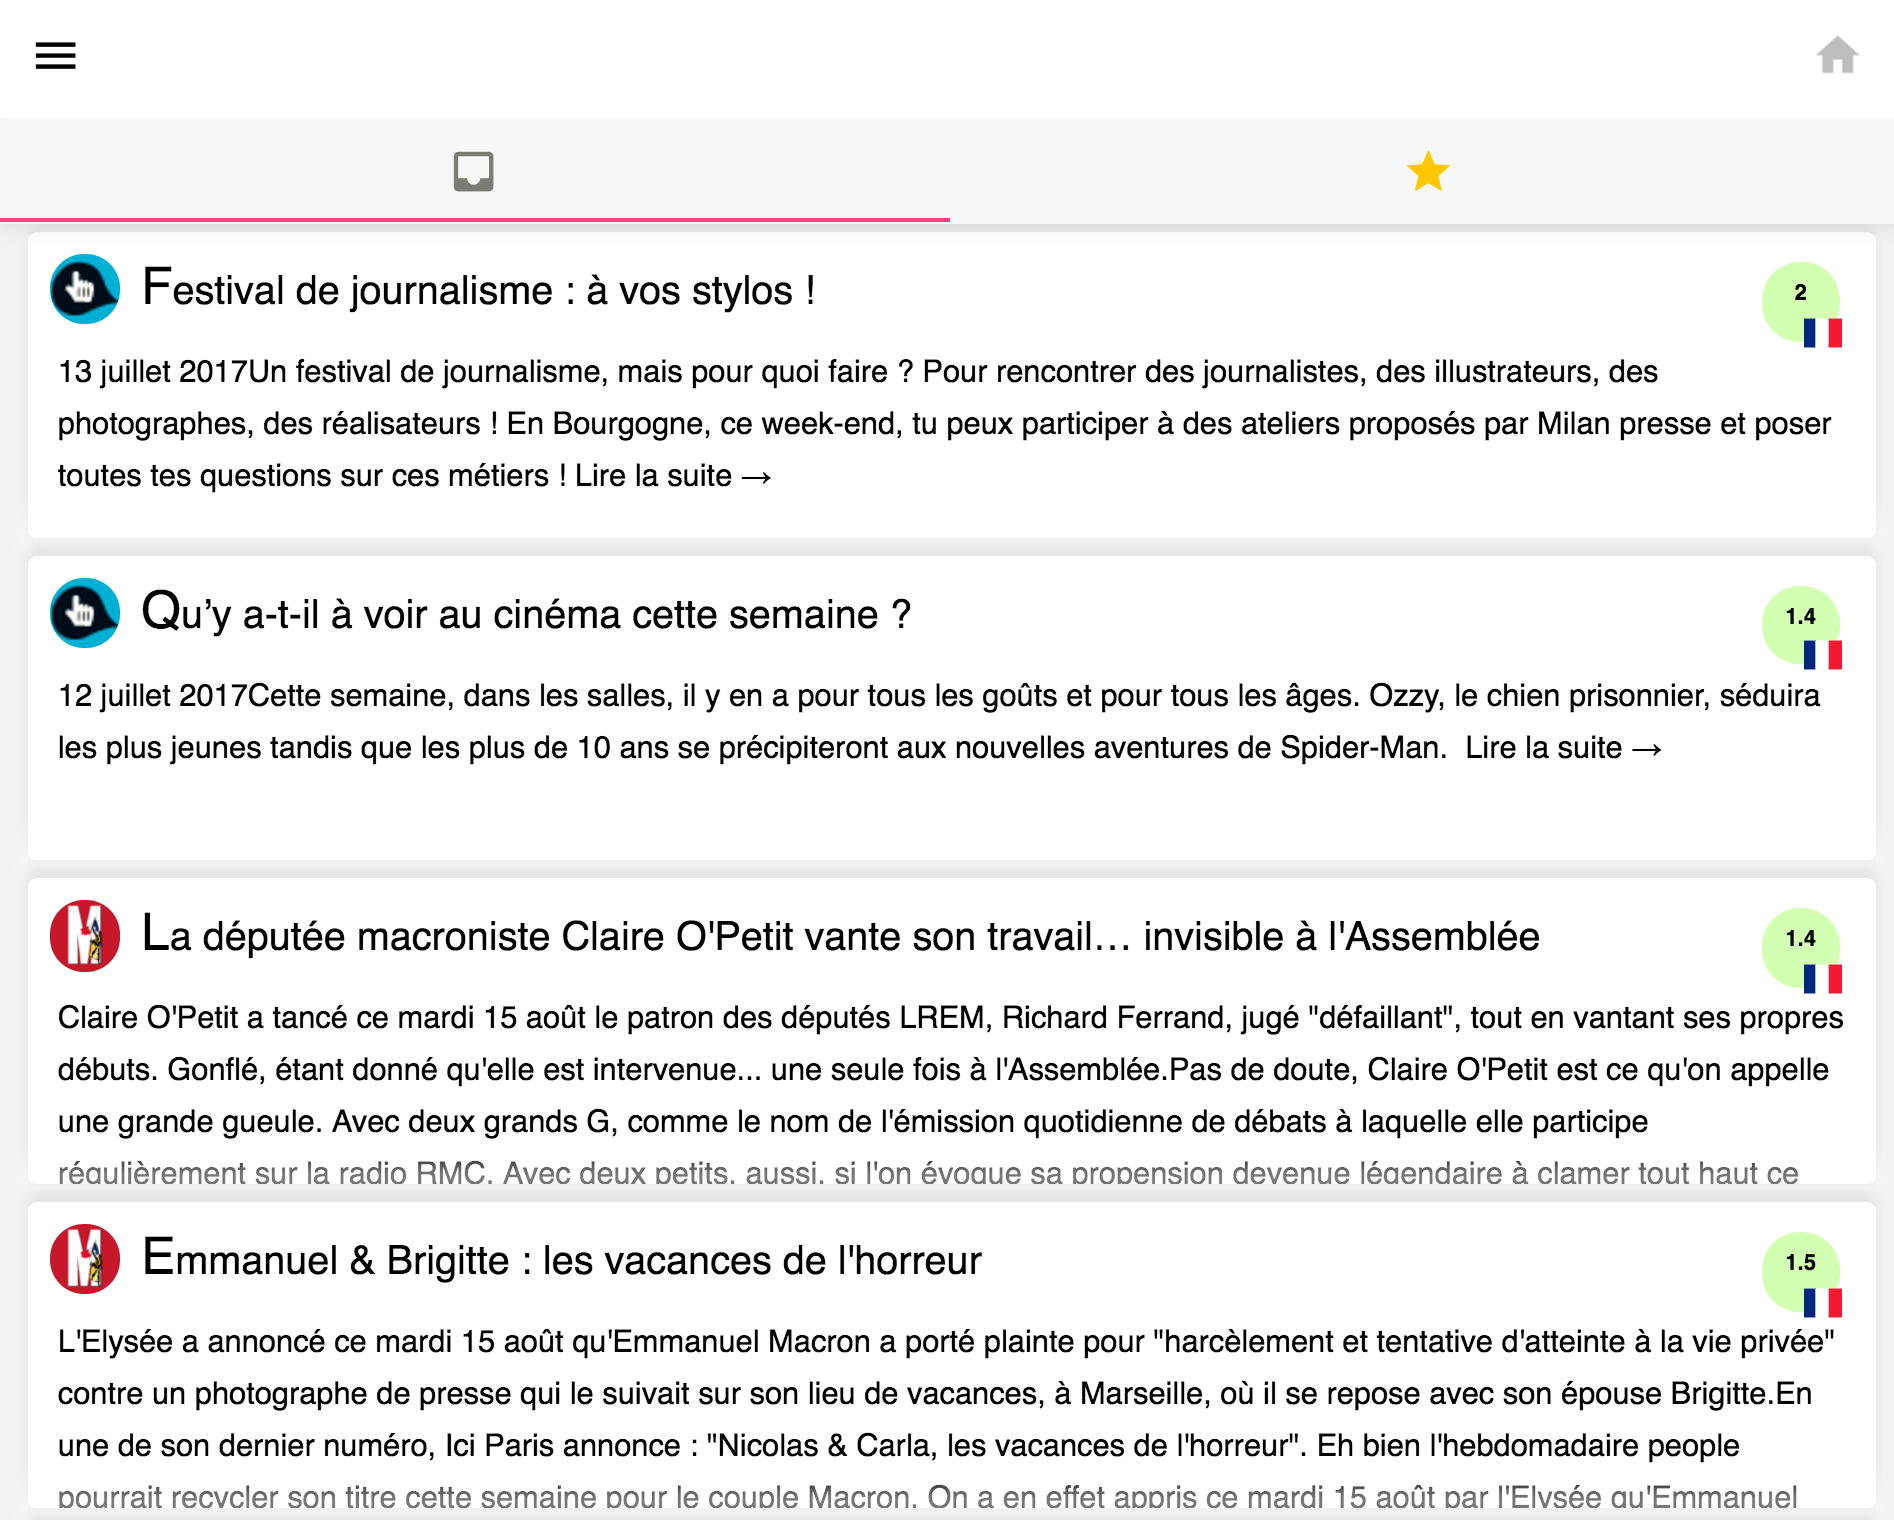
\includegraphics[width=0.95\columnwidth]{figures/article_listing}
  \caption{Article listing presents the source, a summary of the article, and an estimated difficulty level of the article }~\label{fig:registrations}
\end{figure}


\subsection{The Text Reader}

The goal of the reader is to make reading as facile as possible. To do this we optimized for the most frequent action that a reader might want to perform. Translating a word. 

We explored several types of interactions and we settled on the following: a user clicks on a word, a translation is inserted right after the word, as Figure \ref{fig:translated_word} illustrates: 

\begin{figure}[h!]
\centering
  
\includegraphics[width=0.8\columnwidth]{figures/translated_word}
  \caption{A translated word is inserted after the tapped word.}~\label{fig:translated_word}
\end{figure}

Ohter alternatives that we explored and eventually dropped for each had disadvantages were: 
\begin{itemize}

  \item Showing a popup of the translation, and then hiding it again. This had the disadvantage of in the case of a more difficult sentence the reader forgetting the word at the begining of the sentence by the time he arrived to the end, and having to re-translate it. 

  \item Piggybacking on the native selection mechanism. We experimented with allowing the learner to select a word in the same way this is normally done on the corresponding platform and to add the translation as an option in the corresponding popup menu. The problem with this is that native selection is slow, requiring about one second before it is activated. 
\end{itemize}


\subsubsection{Chaining Multiple Adjacent Translations}
The user can chain a few consecutive words into a single translation by simply tapping adjacent words which are automatically merged in a translation bubble (Figure \ref{fig:translation_extension}). This is useful for collocations and in cases where by expanding the translated set of words the precision of the translation increases. 

    \begin{figure}[h!]
    \centering
      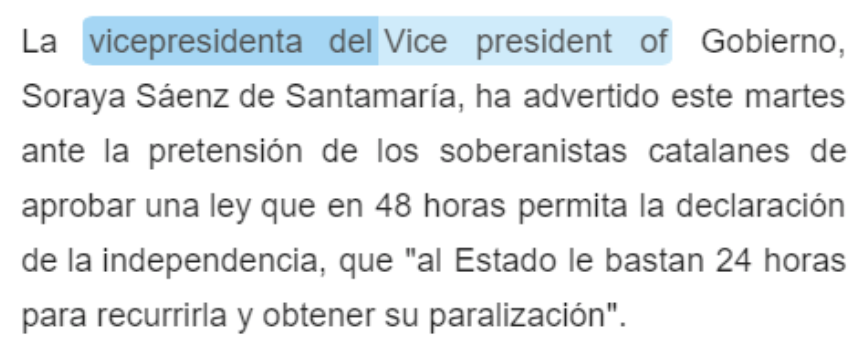
\includegraphics[width=0.8\columnwidth]{figures/translated_words1}
      
\includegraphics[width=0.8\columnwidth]{figures/translated_words2}
      \caption{When adjacent words are tapped the translation bubble is extended accordingly}~\label{fig:translation_extension}
    \end{figure}

This minimalistic interaction model serves a double purpose - it enables and eases the translation of several chained words but it discourages users from translating entire sentences or phrases. This is good because it is in line with the recommendations of the literature (e.g. Renandya argues that extensive reading should discourage intensive use of translations\cite{renadya07-power}) but also because it reduces the amount of characters which are being translated by the learner (and thus the costs of the system, since some of the translation services have a per-character fee). 

One of the limitations of this interaction is that it is not clear (at least at the moment) how to expand it for the situations in which expressions are present that are composed of words which are not adjacent (e.g. particle verbs in German and Dutch).


\subsubsection{Alternate Translations}
Due to the limitations of machine translations, it can be the case that multiple translations might seem appropriate in a context. In such a case the system will insert the most likely alternative but allow the reader to discover the others. With a click on the translation, a drop-down menu appears in which alternatives are presented. Besides the alternatives, there's also an input box in which the learner can provide is own version if none of the offered alternatives are correct. 

Based on telemetry from the system it seems that \ml{must check and limit this only to the french-learning kids} the alternative translations menu is opened one in every eight translations. 

\begin{figure}[h!]
\centering
  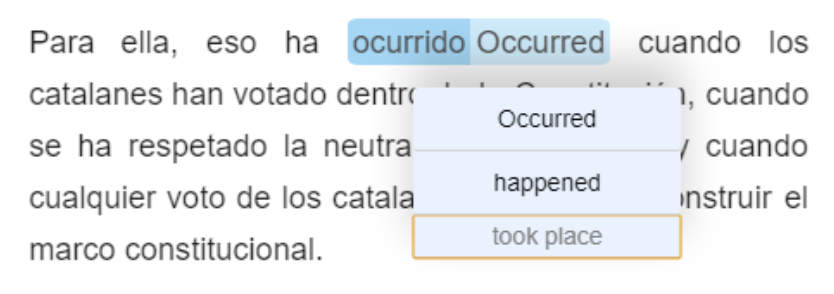
\includegraphics[width=0.8\columnwidth]{figures/translation_alter_menu}
  \caption{A translated word is inserted after the tapped word.}~\label{fig:registrations}
\end{figure}

\subsubsection{Pronounciation}
One of the important features, which was suggested by early beta-testers and added to the system after that was the option of having pronounciation of the given word. Currently this is the action associated with tapping on the highlighted translated word. Although no user has yet complained about it, this means that a user can not pronounce word without it being translated first. It might also be that for some languages this is more important than for others, and we just did not have users learning those languages (e.g. Danish is notoriously hard to pronounce). In the future we plan to expand the interaction modes to allow pronounciation 

\subsection{The Vocabulary Trainer}

Given the list of words that a user does not know we can generate exercises for them based on their past readings.

The various interactive elements (IEs) that are present in this exercise (and in some of the other exericses are): 

\begin{description}
	\item A hint button (IE1) --
	\item Check the answer (IE2) -- 
	\item Word pronunciation (IE3) -- 
	\item Control over the exercise card: report or delete the exercise (IE4) -- 
	\item Input box (IE5) -- 
\end{description}

\begin{figure}[h!]
\centering
  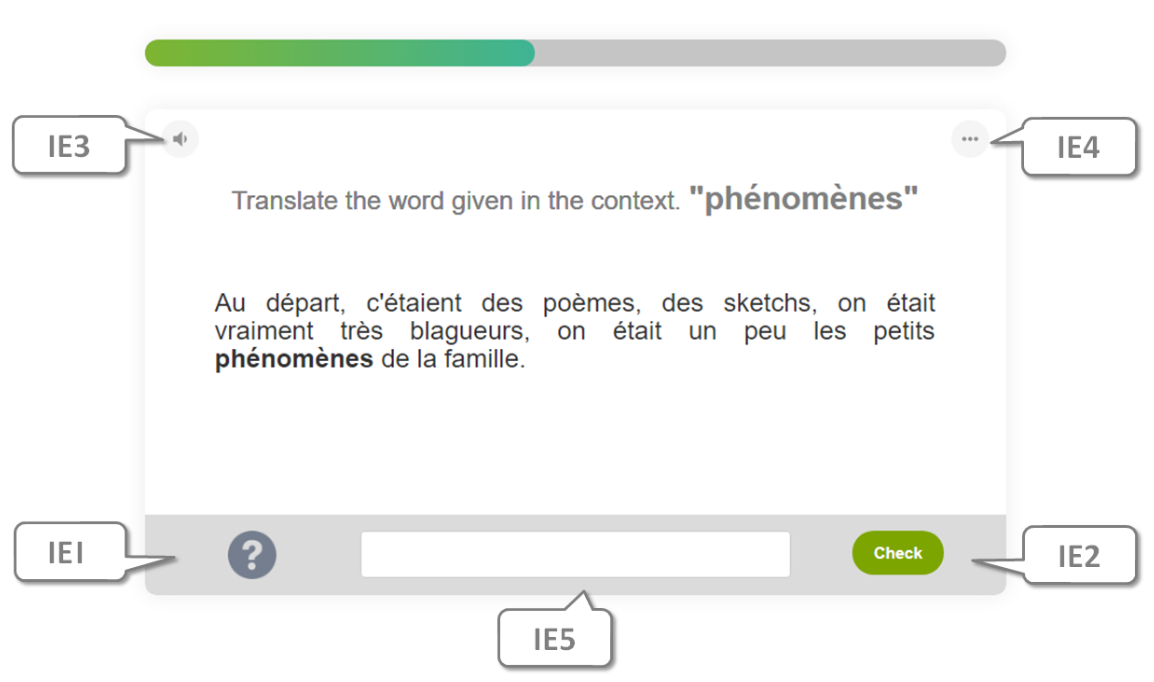
\includegraphics[width=\columnwidth]{figures/exercise_translate}
  \caption{One of the exercise types with which the user is presented. Multiple exercise types are taken from the users past reading context}
\end{figure}

\subsubsection{Words Good for Study}

The words good for study are the ones that are either starred by the user, or are important and of quality based on a set of heuristics. 

\begin{description}

  \item [Important words] are the ones which appear frequently in the language. 
  
  \item [Quality words] are most of the times single words or at most two adjacent words. They come with a context which is not too short but not too long. 

\end{description}

\subsubsection{Scheduling Exercises}

The scheduling algorithm is based on an adaptive, response-time-based scheduling algorithm [was developed] to increase the efficiency of perceptual learning by Mettler et al. \cite{Mettler14-ARTS}. After evaluating several alternative scheduling strategies we settled on the Mettler one since it has been proven to have gains with both familiar, seen items as well as with new, unseen instances and the benefits of adaptive scheduling were present at an immediate test as well as at a delay \cite{Mettler14-ARTS}.



One of the problems with this is that sometimes the context is too long and sometimes 


\subsection{Translation Service}

The translations are provided by our server. The main advantage of this indirection is that this allows the server to track the words that are looked up and the context (sentence) in which they are being looked up. This information is then used for estimating learner knowledge and for generating later personalied exercises. 

To avoid depending on a single service and to also increase the likelihood that at least one of the alternative translations is the correct one, the translation service dispatches in parallel requests to at least three third party translation APIs: Google Translate, Microsoft Translate, and Glosbe -- a free translation API. The first two provide contextual translations and multi-word translations, while the third is a simple dictionary. 

The dependency of the translation service on multiple third party APIs allows for a higher reliability and a chance to guarantee a low response time: when a service is down or too slow to respond, the results from it are ignored.

\subsection{The Teacher Dashboard}

Although not the focus of this paper, the system has also a dashboard for the teacher. The teacher can see the history of what his students have read. 






